%  !TEX root = ../main.tex

\section{Introduction}
Automatic speech recognition (ASR) enables computers to transcribe human speech and is essential in a wide range of voice applications such as voice assistants (VAs) and audio transcription APIs~\cite{azureasr,googleasr}.
Prior studies have shown that ASR models are vulnerable to adversarial examples (AEs) that sound benign to humans but are recognized incorrectly by models. 
As stealthiness is a basic requirement for AEs, existing works largely focus on reducing the audibility of AEs so that they might not cause human suspicion when being heard~\cite{schonherr2018adversarial,qin2019imperceptible}. In addition, the class of inaudible attacks~\cite{zhang2017dolphinattack,sugawara2020light} avoids being perceived by human ears using high-frequency ultrasound/laser.
However, few of them have considered attacks in user-present scenarios, where users may notice unexpected events of the ASR service and can mitigate the attack's consequence.
For instance, though AEs and inaudible attacks may not sound suspicious, a voice assistant will always provide feedback (e.g., vocal prompt or LED blinking) after receiving voice commands. Alert users may still notice the false wake-up or abnormal feedback caused by an attack and speak remedy commands to correct the mistake, limiting the attack's impact in real life.


\begin{figure}
    \centering
    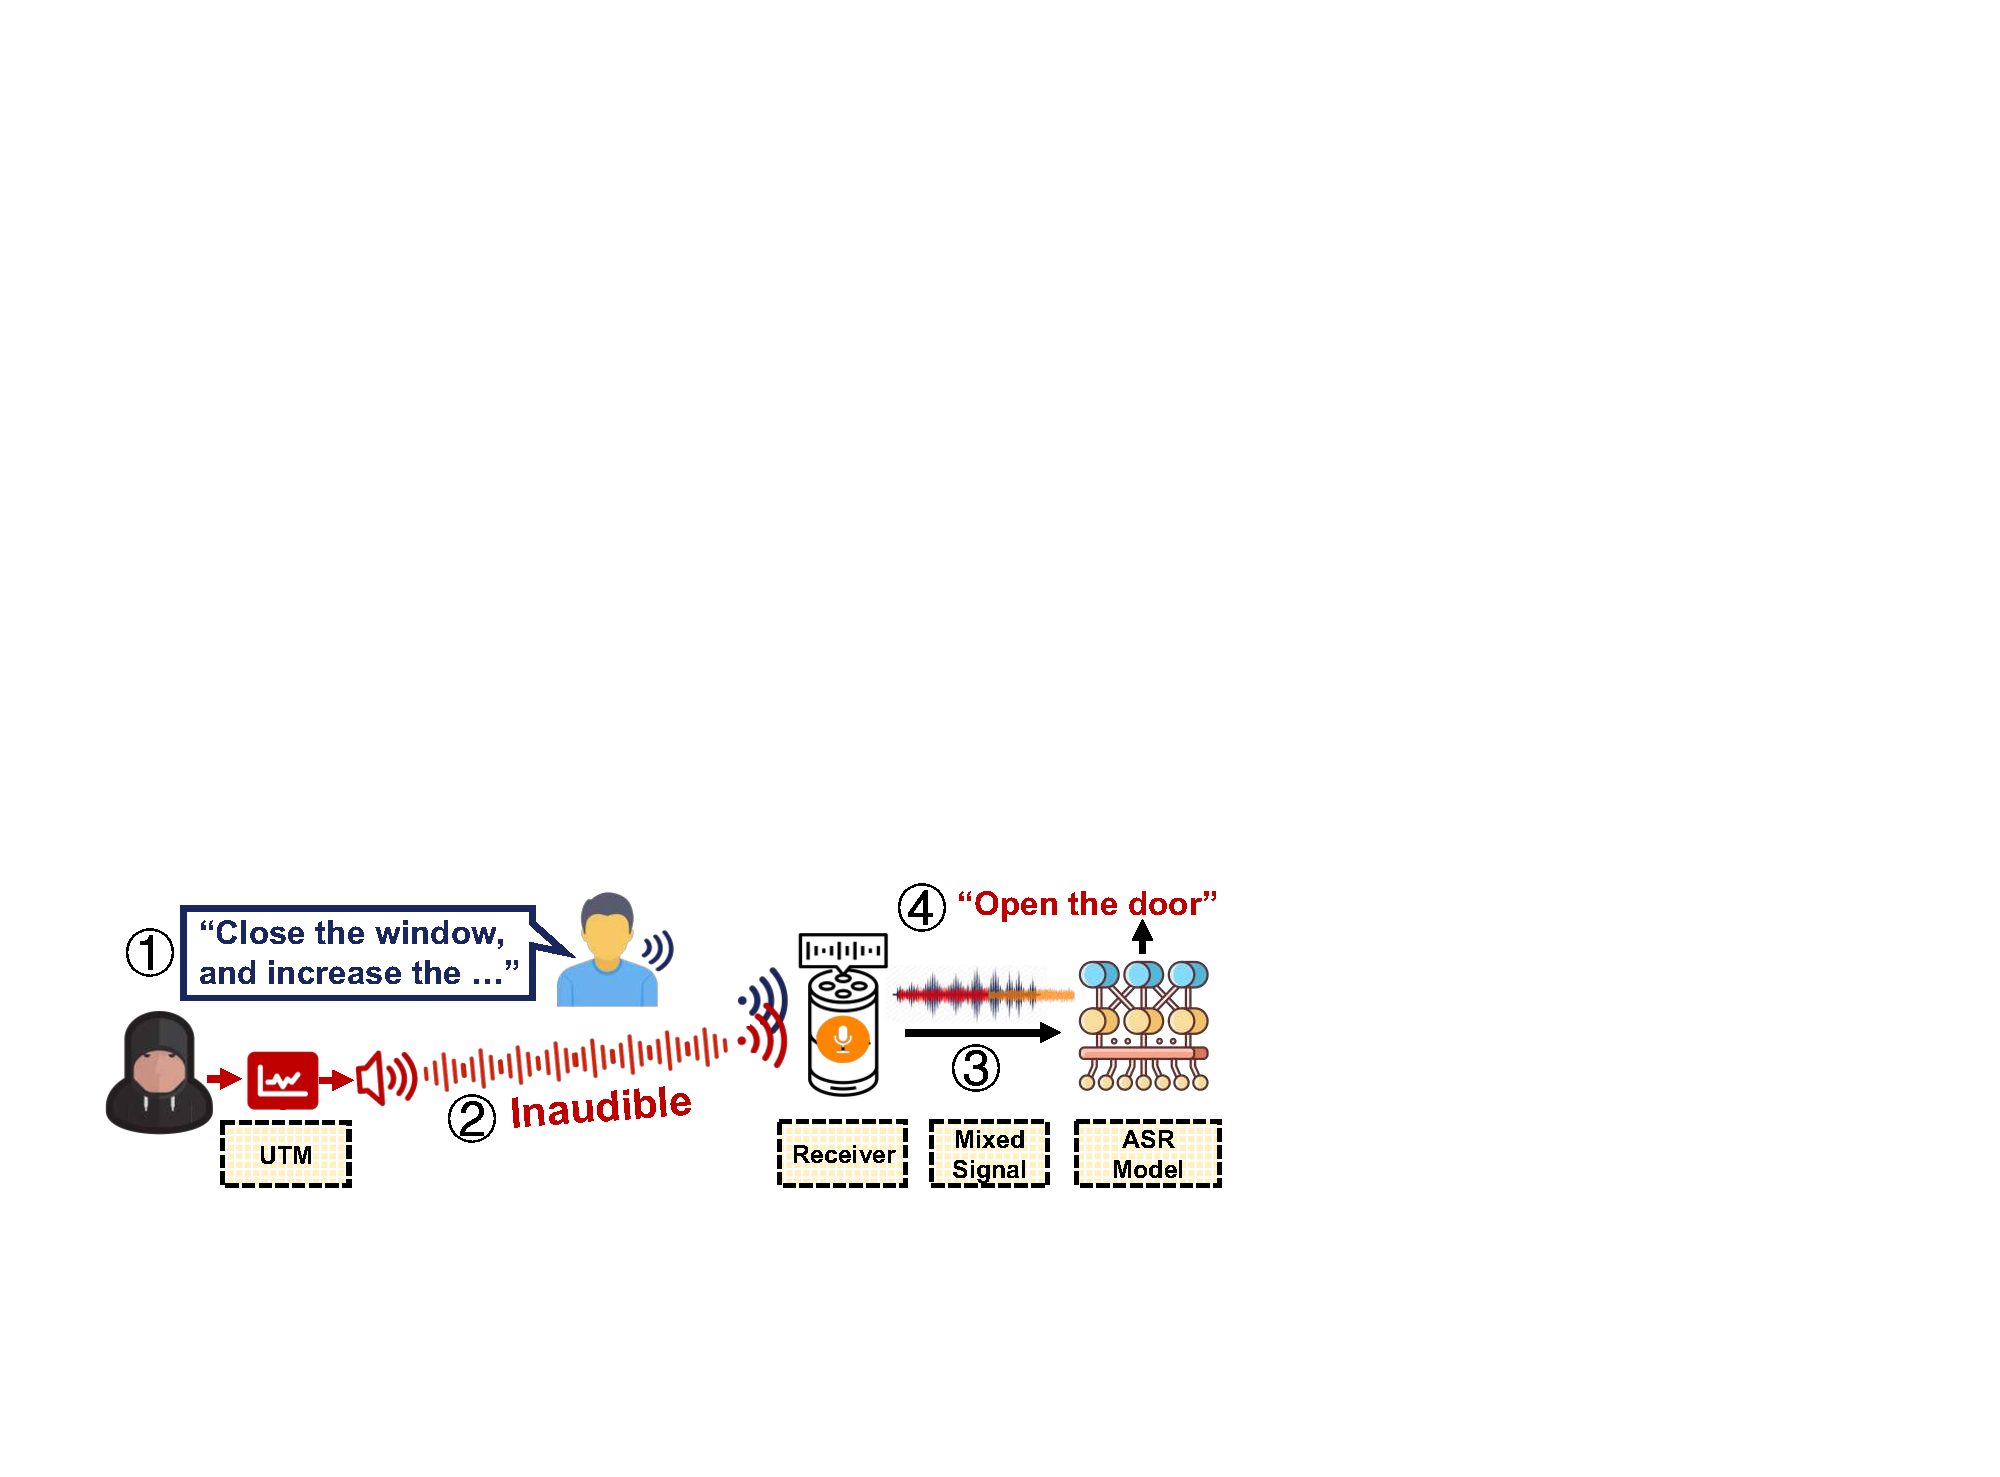
\includegraphics[width=0.48\textwidth]{fig1-7.pdf}
    \caption{\ding{172}When a user uses the ASR service, \ding{173}an adversary injects inaudible adversarial perturbations crafted based on the ultrasonic transformation model (UTM) into a receiver. \ding{174}The mixed signal of the user command (blue) and demodulated perturbations (red \& yellow) can \ding{175}fool the ASR model into the adversary-desired intent.}
    \label{fig:fig1}
    \vspace{-15pt}
\end{figure}


In this paper, we aim to propose \alias\footnote{Demo: https://sites.google.com/view/Vrifle}---an \textit{inaudible adversarial perturbation} (IAP) attack that can extend to this scenario. Its basic idea is to inject IAPs while the user speaks to the ASR service and alter the recognition result in real time, as shown in Fig.~\ref{fig:fig1}. Since the voice assistant itself is responding to user commands (e.g., LED blinking), tampering with the user's speech is less noticeable at this time. 
\blue{
But such a user-present scenario also imposes higher requirements on attack stealthiness because users are more sensitive to environmental sounds while using ASR services. 
Moreover, given that adversaries have no prior knowledge of user's speech content and timing, this critical scenario necessitates that \alias exhibits a high level of universality to guarantee the achievement of the adversary-desired intent in any context.
Therefore, we envision \alias as a truly inaudible and robust framework for real-time IAPs delivery, which can also address variable user factors, such as speech content, vocalization time, speech volume, and environmental conditions, while remaining physically effective even at long distances or using portable/everyday-life devices.
Overall, materializing \alias that attains the above goals is challenging in three aspects.}


\begin{itemize}[leftmargin=*]
\item \textit{How to achieve adversarial perturbations that are \textbf{universal} while \textbf{completely inaudible} to \textbf{user auditory}?}
\end{itemize}

The trade-off between universality and stealthiness has been a long-standing challenge in audio AE attacks. Almost all previous works have prioritized stealthiness and introduced imperceptibility constraints during optimization, such as $\epsilon$ and L2-Norm~\cite{carlini2018audio}, or by adjusting audio forms, e.g., designing it as short pulses~\cite{guo2022specpatch}. Nonetheless, this greatly compromises the universality of adversarial perturbations and they are still audible and can be heard when users are nearby.
We seek to implement an inaudible adversarial perturbation beyond the human auditory range (20~Hz$\sim$20~kHz) in an ultrasound-based attack manner~\cite{zhang2017dolphinattack},
which can make microphones receive our IAP by exploiting their inherent nonlinearity vulnerability. As such, IAPs are no longer limited by stealthiness constraints, holding a vast optimization space with more feasible solutions. 
Unlike the audible-band perturbations devised to be short to mitigate user auditory, our IAPs enable the adversary to significantly increase their length, which further expands the optimization scope and facilities highly universal attacks.


\begin{itemize}[leftmargin=*]
\item \textit{How to alter the recognition of user speech in real time despite the presence of \textbf{user disruption}?}
\end{itemize}


Although we have bypassed \textit{user auditory}, realizing such an attack against ASR in real time faces a few more challenges. 
\blue{
\textit{User disruption} cannot be ignored in this scenario, which includes: \ding{202} The user's speech can disrupt the intent of IAPs when both audio signals are superimposed. While universal AEs~\cite{li2020advpulse,guo2022specpatch} are shown to resist this case, our preliminary investigation validates that direct ultrasound-based attacks will fail due to such interference. \ding{203} User commands can be much longer (e.g., 5s) than 0.5s audible-band short perturbations that affect only a few input frames, thus the exceeded user instructions will impact the entire ASR transcription. \ding{204} Users may notice that malicious behavior being executed and therefore block the attack by issuing remedy commands. 
In addition, there are user-induced factors that make \textit{user disruption} more complex and can compromise IAPs' effectiveness, including unpredictable content and timing of user speech, as well as the influence of the user's environment and speaking habits on speech reverberation and loudness.}

To address these issues, we augment the optimization process of IAPs by using multiple speech clips in public corpus, introducing randomness within the preset time range, as well as considering the various user's speech loudness and reverberation. Thereby, \alias can be applied in a content-agnostic, synchronization-aided, user factors-robust manner. Moreover, we overcome \textit{user disruption} by materializing both silence and universal perturbations in the targeted manner to ensure the arbitrary utterance length cannot pose impacts on adversary-desired intent, without requiring any knowledge.
Based on the above design, adversaries can present two more hidden attack strategies, involving \textit{No-feedback Attack} and \textit{Man-in-the-middle Attack} in the threat model.


\begin{table}\centering
    \small 
    \renewcommand{\arraystretch}{0.5}
    \renewcommand\tabcolsep{5.5pt}
    \begin{threeparttable}[t]
    % \renewcommand{\TPTminimum}{\linewidth}
    \setlength{\abovecaptionskip}{5pt}% 
    \setlength{\belowcaptionskip}{0pt}%
    
    \caption{Compared with existing works}
    \begin{tabular}{@{}lcccc@{}}
        \toprule
        \textbf{Method} & \textbf{Constraint$^\ddagger$} & \textbf{Auditory$^\natural$}  & \textbf{Disruption$^\star$} 	& \textbf{Dist.$^\dagger$}\\ \midrule
        Carlini.~\cite{carlini2016hidden}  &   $\relbar$   &  Noise  & \xmark    & 1.5m      \\ \midrule
        Abdullah~\cite{abdullah2019ndss} &   $\relbar$   &  Noise  & \xmark    & 0.3m      \\ \midrule
        CW~\cite{carlini2018audio}  &  L2-norm, $\epsilon$   &  Speech  & \xmark    & \xmark       \\ \midrule
        Schönherr~\cite{schonherr2018adversarial} &  Psyc.   &  Speech  & \xmark    & \xmark       \\ \midrule
        Comman.~\cite{yuan2018commandersong} &  $\epsilon$   &  Song  & \xmark    & 1.5m  \\ \midrule
        Qin.~\cite{qin2019imperceptible}  &  Psyc.   &  Speech  & \xmark    & $\relbar$  \\ \midrule
        Meta-Qual~\cite{chen2020metamorph}  &  L2-norm, $\epsilon$   &  Song  & \xmark    & 4m  \\ \midrule
        FakeBob~\cite{chen2021fakebob} &  $\epsilon$   &  Speech  & \xmark    & 2m  \\ \midrule
        AdvPulse~\cite{li2020advpulse} &  L2-norm, $\epsilon$   &  Ambient  & \ding{119} & 2.7m  \\ \midrule
        % FenceSitter~\cite{deng2022fencesitter}  &  SNR   &  Ambient  & \cmark   & 3m  \\ \midrule
        SpecPatch~\cite{guo2022specpatch} &  L2-norm   &  Pulse  & \ding{119}  &  1m    \\ \midrule
        \textbf{Ours}   &  \textbf{None}   &  \textbf{Inaudible}  &  \ding{108}  & \textbf{10m}  \\ \bottomrule
        % https://tex.stackexchange.com/questions/42619/xmark-that-complements-the-ams-checkmark
        \end{tabular}
        \begin{tablenotes}[flushleft]
        \item[] \vspace{-2pt}\hspace{-2pt}\small 
        (i) $\ddagger$: The constraints used to guarantee imperceptibility during optimization. ``$-$'' means the method only considers incomprehensibility to humans. $\epsilon$ means limiting the absolute magnitude of perturbations with a constant $\epsilon$. $L_2$-Norm means adding an $L_2$-Norm term in the objective function. ``Psyc.'' means psychoacoustic hiding. ``None'' means no stealthiness constraints. 
        (ii) $\natural$: The objective \textit{\textbf{user auditory}} of AEs. Ambient means ambient sounds.
        (iii) $\star$: \ding{108}: fully tackles \textit{\textbf{user disruption}}. \ding{119}: tackles case \ding{202}. \xmark: fails by \textit{\textbf{user disruption}}.
        (iv) $\dagger$: \xmark: the attack is not physically available. $\relbar$: not reported.
      
        \end{tablenotes}
        \vspace{-10pt}
    \label{tab:compare}
    \end{threeparttable}
\end{table}



\begin{itemize}[leftmargin=*]
\item \textit{How to guarantee inaudible adversarial perturbations are \textbf{physically effective} after ultrasonic delivery?}
\end{itemize}

Though inaudible attacks have demonstrated voice command injection using ultrasound and laser~\cite{sugawara2020light}, \textit{it is unknown whether fine-grained IAPs can be delivered via such signals} as the ultrasound channel is reported to be lossy and distorted~\cite{li2023learning}. Thus, maintaining the effectiveness of IAPs after undergoing a series of modulation, transmission, and demodulation processes in the physical world is not trivial based on prior AEs~\cite{schonherr2020imperio}. Ultrasound is intrinsically distinct from audible sounds in the high-directional propagation and varying soundfield. Additionally, the nonlinear distortion, anomalous noises, and hardware-induced instability that are unique to ultrasound make existing acoustic channel modeling methods inapplicable.

To overcome the challenge, we make the first attempt to establish an ultrasonic transformation model, which consists of tackling variable ultrasound-induced anomalous noises, obtaining ultrasound frequency response (UFR), and enabling location-variable attacks. 
Based on this transformation, we can precisely estimate \alias's pattern of ultrasonic delivery during its optimization, thereby making it physically effective and survive long-distance delivery. Moreover, to enable more covert IAP attacks with portable devices and off-the-shelf loudspeakers, we implement a narrow bandwidth upper-sideband modulation (USB-AM) mechanism to ensure the attack range and inaudibility of \alias with simplified devices.

Tab.~\ref{tab:compare} compares \alias with several existing works. 
We conduct extensive experiments in both digital and physical worlds to evaluate \alias's effectiveness under various configurations (e.g., extend attack range to 10m) and robustness against six kinds of defenses. Our single silence IAP muting up to 27,531 unseen user utterances, likewise, universal IAP altering 18,956, proving \alias's universality. 
\blue{Our design also expands the attack methodology to more covert portable attack devices and everyday-life loudspeakers, enabling the \alias delivery in a stealthier form.} 
Our contribution can be summarized as follows:

\begin{itemize}[leftmargin=*]
    \item To the best of our knowledge, \alias is the first universal inaudible adversarial perturbation attack that can extend to scenarios when users use ASR services, revealing a new attack surface against ASR models. \alias is completely inaudible, holds vast optimization space, and enables long-range attacks (10m).
    \item We make the first attempt to establish an ultrasound transformation model, which overcomes the unique challenges in the ultrasound channel and precisely characterizes it, enabling our fine-grained IAPs delivery to be physically effective.
    \item We conduct extensive experiments under various configurations in the digital and physical world to validate the effectiveness, robustness, and universality of \alias, and validate the attack using portable/everyday-life devices.
    
\end{itemize}
